%%
%% This is file `sample-sigconf.tex',
%% generated with the docstrip utility.
%%
%% The original source files were:
%%
%% samples.dtx  (with options: `sigconf')
%% 
%% IMPORTANT NOTICE:
%% 
%% For the copyright see the source file.
%% 
%% Any modified versions of this file must be renamed
%% with new filenames distinct from sample-sigconf.tex.
%% 
%% For distribution of the original source see the terms
%% for copying and modification in the file samples.dtx.
%% 
%% This generated file may be distributed as long as the
%% original source files, as listed above, are part of the
%% same distribution. (The sources need not necessarily be
%% in the same archive or directory.)
%%
%% The first command in your LaTeX source must be the \documentclass command.
\documentclass[sigconf,10pt]{acmart}

\usepackage{amsmath}
\usepackage{algorithm}
\usepackage[noend]{algpseudocode}

\settopmatter{printfolios=true}

\pagestyle{plain} % removes running headers
\settopmatter{printacmref=false} % Removes citation information below abstract

%%
%% \BibTeX command to typeset BibTeX logo in the docs
\AtBeginDocument{%
  \providecommand\BibTeX{{%
    \normalfont B\kern-0.5em{\scshape i\kern-0.25em b}\kern-0.8em\TeX}}}

%% Rights management information.  This information is sent to you
%% when you complete the rights form.  These commands have SAMPLE
%% values in them; it is your responsibility as an author to replace
%% the commands and values with those provided to you when you
%% complete the rights form.
% \setcopyright{acmcopyright}
% \copyrightyear{2019}
% \acmYear{2019}
% \acmDOI{10.1145/1122445.1122456}

%%
%% Submission ID.
%% Use this when submitting an article to a sponsored event. You'll
%% receive a unique submission ID from the organizers
%% of the event, and this ID should be used as the parameter to this command.
%%\acmSubmissionID{123-A56-BU3}

%%
%% end of the preamble, start of the body of the document source.
\begin{document}

%%
%% The "title" command has an optional parameter,
%% allowing the author to define a "short title" to be used in page headers.
\title{Pi-Tree: A Multidimensional Learned Index}


\author{Adam Jaffe}
\email{ajaffe@uwaterloo.ca}
\affiliation{
  \institution{University of Waterloo}
  \city{Waterloo}
  \state{Ontario}
}

\author{Xiyang Feng}
\email{x74feng@uwaterloo.ca}
\affiliation{%
  \institution{University of Waterloo}
  \city{Waterloo}
  \state{Ontario}
}



%%
%% The abstract is a short summary of the work to be presented in the
%% article.
\begin{abstract}
  This is my abstract, so it is not concrete yet. It cannot yet be used
  in the constructions of domiciles for human habitation.
  % TODO
\end{abstract}


%%
%% This command processes the author and affiliation and title
%% information and builds the first part of the formatted document.
\maketitle

\section{Introduction}

Analytical database engines store and process queries on large volumes of data.
These systems scan and filter large volumes of data to execute queries.
Multidimensional range queries are a type of query defined by 
intervals in all or some of the columns and are interested in all data items
that are within all the given intervals. Multidimensional range queries that do not specify
an interval for at least one column are called partial range queries, whereas queries that specify
an interval for all dimensions are called complete range queries.
Multidimensional range queries are a common task for many applications.
For instance, they are used to query sensor data across a section of time and space, as well as in business
intelligence, scientific data and data science \cite{ModernMDRQ}.

With the explosion of analytical data comes the need to answer multidimensional range queries
quickly on large datasets. Multiple approaches have been taken to perform better than
fully scanning the dataset, which is quite wasteful if selectivity
of the query is low. If queries are very selective in one column, then sorting the data
according to that column and building a B-Tree on that column can be a good approach. 
Another approach is to use a multidimensional index, which uses data from multiple dimensions
in its structure. 

In this paper we present Pi-Tree, a learned multidimensional index designed for
in-memory multidimensional range queries capable of indexing
data of arbitrary dimension. PiTree extends in a natural way the recursive model index (RMI) structure
from the original learned index paper to a multidimensional space.
Our main contributions are:
\begin{enumerate}
  \item The design and implementation from scratch of the Pi-Tree multidimensional learned index in C++
  % TODO highlight benchmark results
  \item A thorough evaluation of Pi-Tree against an R*-Tree and kd-Tree 
  \item A discussion of future work to improve the performance of Pi-Tree
\end{enumerate}

The rest of this report will be structured as follows.
Section 2 covers related work. Section 3 and 4 describes
work done on learned indices in the single dimensional case.
Section 5 describes the design and implementation
of Pi-Tree. Section 6 highlights our benchmarking results. Section 7
outlines potential future work to be done.

\section{Related Work}

Both the original learned index work, and SageDB
proposed applying a learned based approach to multidimensional indexing,
but neither provided details \cite{Learned_Index,SageDB}.
Recently, a multidimensional leanred index strucuture called Flood has been proposed  \cite{Flood}. 
Flood is most similar to a grid file
\cite{Grid-File}, which partitions the data in a grid-like fashion.
Flood has a global axis-aligned projection and partitioning scheme,
while Pi-Tree projects and partitions at a per-node basis. 

Many other multidimensional indexing schemes have been proposed
over the past decades. Three main approaches have been taken:
space filling curves, tree-based structures, and bucketing are three popular approaches
to build multidimensional indexes. Space filling curves, such as the Z-order,
can be used to define an order on $n$-dimensional space, which can then be indexed using 
single-dimensional methods \cite{UB-Tree}. 
A complication of this approach is that points that are close in
n-dimensional space are not necessarily close together on the curve.
Tree-based structures can be though of as the multidimensional extension of B-Trees.
There are a variety methods that take this approach, such as R-Trees, kd-trees
\cite{R-Tree,R*-Tree,kd-Tree}.
Bucketing coarsely partitions the data space, which are then scanned and filtered to produce
the result set \cite{Grid-File,Flood}.
R-Trees are popular for indexing spatial data,
since they are capable of indexing regions and not only points \cite{R-Tree,R*-Tree}.
For instance, PostGIS uses an R-Tree for indexing \cite{PostGIS}.
However, as shown in the benchmarks, the R-Tree does not excel at 
indexing points, especially in higher dimensions.

Kd-Trees are popular for nearest neighbour queries 
and can also perform range queries \cite{kd-Tree,ModernMDRQ}.
Pi-Tree, with the round-robin projection policy, can be though of as a combination
of a kd-Tree and an RMI \cite{Learned_Index}. 
An extension of the kd-Tree, called the cracking kd-tree adaptively
changes its structure while processing queries in order to improve 
the performance for subsequent queries \cite{CrackingKD-Tree}.
These approaches use only local policies and do not incorporate the global distribution
of the data.


\section{Background}

\subsection{Recursive Model Index}

The recent work by Kraska et al. on learned indexes
has cast the problem of single dimensional indexing in a new light \cite{Learned_Index}.
Their key insight is that given the empirical cumulative distribution function
of the dataset, in most cases, a very compact index can be constructed. 
The index structure they proposed is called the recursive model index (RMI) and they
demonstrated that it can take orders of magnitude less memory
than a classic B-tree while simultaneously providing similar throughput.

There are two key ideas behind RMI that made it so successful.
First is that overfitting is not an issue, unlike almost all other machine learning 
applications. In a non-dynamic indexing setting, the model does not need extrapolative
power, allowing simpler models to be used.
The latter specifies that one complex model for the CDF is impractical due to large inference times
and memory size, and that a more fruitful approach is to 
use a hierarchy of models. The root model and internal models are used to route
to more specific models, which are trained on smaller segments of the dataset. 
Researchers have tried different types of models in the hierarchy, including neural nets,
but the consensus seems to be that linear models perform the best due
to their small memory footprint and very quick inference time. % CITE learned index blog/argument, ALEX, etc.
Linear models are simply comprised of two floats $a$ and $b$ and inference
can be done with one multiplication, one addition, and an application of floor:
$y = \lfloor ax + b \rfloor$.

The leaf models in RMI are used to predict the location of the key in a sorted 
in-memory array. The prediction could be wrong, so a local search around the prediction
is required to find the key, if it exists. In order to speed up the searches,
a max error is maintained to be used for the bounds of the local search.
Since RMI is a clustered index, it is capable of performing single dimensional range searches
by simply finding the left endpoint range, then scanning to the right until reaching the right
endpoint.

\begin{figure}
  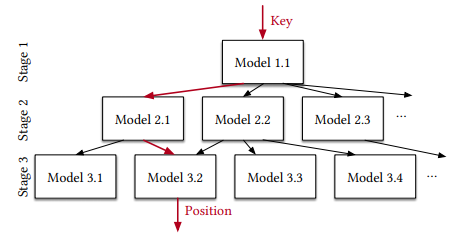
\includegraphics[scale=0.6]{../figures/RMI}
  \caption{RMI\cite{Learned_Index}}
  \label{RMI}
\end{figure}

\section{Single Dimensional Case}

\subsection{Motivation}

\begin{figure}[h]
  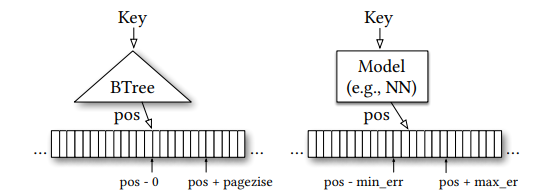
\includegraphics[scale=0.6]{../figures/single-dim-learned-index}
  \caption{Single dimensional learned index \cite{Learned_Index}}
  \label{single-dimensional-learned-index}
\end{figure}

As described in Section 2, the main idea of single dimensional learned index is to replace
the traditional indexing structure like B-Tree with a machine learning model that is able
to learn the underlying data distribution (see Figure 2). For point lookup, the learned index takes a key
as input and predicts the position of the key in the data layout. The prediction does not
necessarily to be exact as a quadratic search is introduced to correct the prediction error.

Theoretically, the point lookup time for single dimensional learned index equals to time
traversing the RMI plus time doing quadratic search. A model that can compute easily and predict
accurately is the key to speed up point lookup. However, there is usually a trade off between
model accuracy and computational cost in machine learning. For example, deep neural net is able
to model complex data distribution but is also extremely expensive to compute. On the other hand,
linear regression only involves one multiplication and one addition, but it only model linear
distributed data effectively. Kraska adopted linear regression based RMI in their single dimension
learned index mainly because the layout of single dimensional data is trivial such that it can be
effectively learned by linear models. However, such property may not hold for high dimensional cases.
Therefore, we think it worth first studying the trade off between model accuracy and model
computational cost. The result may guide us on the choice of models. 

\subsection{Experiment}

We implemented our single dimensional learned index with a two-stage RMI as proposed in 
Kraska's paper \cite{Learned_Index}. The two-stage RMI is configured to be able to accept
any model that takes a key as input and generates a position as output such that we can
plug in any machine learning model as needed. For simplicity, we only test on linear regression
model and neural net with one hidden layer that has eight hidden nodes. A native B-Tree with no optimization is also implemented
as the baseline. All indexing structures are implemented in Python as we do not care about the absolute
performance in single dimensional case as long as the comparison is fair. Moreover, Python provides powerful
machine learning modules such as tensorflow. 

\begin{table}
  \centering
  \begin{tabular}{|c|c|c|c|}
    \hline
     & BTree & Linear Model & Neural Net \\
    \hline
    Avg lookup time(ms) & 8e-6 & 6e-5 & 1e-4 \\
    \hline 
    Avg prediction error & 0 & 0.35\% & 0.22\% \\
    \hline 
    Build time(s) & 0.17 & 24.21 & 80.46 \\
    \hline 
  \end{tabular}
  \caption{benchmark single dimensional learned index}
  \label{table:single-dimensional-learned-index-benchmark}
\end{table}

We benchmark our indexing structures on a random uniformly distributed single dimensional
dataset with 100 thousand data points. Each point is queried exactly once in the benchmark.
All tests are conducted under the same environment as described in Section 5.1. Table 1 shows
the benchmark results of BTree, linear model based RMI and neural net based RMI. Although
BTree appears to be the best indexing structure across all evaluation metrics, we believe the
overhead is mainly due to the tensorflow module as, later on when we finish implementing Pi-Tree
and linear regression in C++, the performance is suprisingly good.

In terms of point lookup speed, neural net is about 20 times slower than linear regression model.
This is as expected since we are using a neural net with 1 hidden layer and 8 hidden nodes which
means for each prediction, neural net needs to do 16 linear regressions. Such high computational
overhead also brings an improvement on prediction accuracy. Neural net reduces the prediction
error (Average distance between prediction and actual position / Total data) by 0.13\%. However,
such improvement is negligible as it can be easily corrected by quadratic search. Model prediction
time becomes the dominant part in point lookup.

\subsection{Lessons Learned}

The success of single dimension learned index lies in the trivial data layout imposed by sorting.
Mispredictions can be effectively corrected without much scan overhead. However, such a feature may
not exist in high dimensional cases. Points that are close in high dimensional space may be projected
far from each other in single dimensional space. Therefore, it is important to carefully design a
projection function which can preserve the relative position between points.

Since high dimensional data is more complex to learn, the choice of machine learning model also
warrants discussion. Although the neural net approach has been shown to be able to predict more accurately, its
large computational overhead is not negligible. The model used in RMI does not necessarily need to
be very accurate but has to be easy to compute. Otherwise, traversing RMI will dominate the lookup.
The rationale behind this is simple. When it takes too much effort to correct the prediction, a better
approach is to simply leave the prediction as is while scanning everything in between. 

\section{Pi-Tree Design}

Pi-Tree is a multidimensional in-memory learned tree index structure for
multidimensional range queries. Currently, only complete range queries are supported.
Partial range queries are possible to support but are not included in this report. 
Pi-Tree indexes a static dataset and does not support dynamic inserts, deletes,
although we believe it is possible to extend Pi-Tree to allow dynamic inserts and deletes,
in the same way ALEX built upon the original RMI structure to achieve this functionality. % CITE ALEX

The datapoints, all of dimension $D$, are stored as one contiguous in-memory array.
Nodes in Pi-Tree are comprised of a projection onto a single dimension, which it uses to
sort data points, and a linear regression model which models the CDF of a segment of the data.
Internal nodes use the linear model to select a child node to route to.
Leaf nodes use the linear model to find the relevant data point. 
Pi-Tree is configurable with two parameters: the $pageSize$, 
which bounds the number of data points
a leaf node indexes, as well as $maxFanout$, which bounds the fanout
of an internal node.

\subsection{Node Structure}

\begin{figure}
  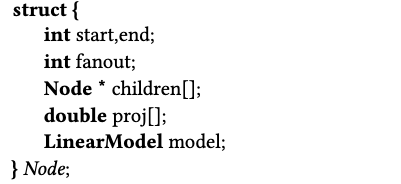
\includegraphics[scale=0.5]{node_structure.png}
  \caption{Pi-Tree Node Structure}
  \label{Pi-TreeNode}
\end{figure}


Each node $n$ is responsible for indexing the range of the data array with indexes in $[start_n, end_n)$.
Nodes contain a projection vector $proj_n$ of the same dimension of the data
which it uses to sort the range of data it indexes. 
To be precise, if $d_1, d_2$ are two datapoints, the node will 
sort $d_1$ before $d_2$ if $d_1 \cdot proj_n < d_2 \cdot proj$.
Pi-Tree uses a policy to select a projection on a per-node basis. In this report,
we only tested a policy which chooses a dimension to project onto in a round-robin
fashion, similar to how a kd-tree selects which dimension to split at each depth.
In particular, if a node is at depth $h$, then its
$D$ dimensional projection vector is the standard basis vector $e_{h \% D}$ that has components 
$$a_j = \begin{cases} 
  1 & j \equiv h \mod D \\
  0 & otherwise
\end{cases}
$$
for $j=1, \cdots, D$ and dimension $D$. Although for this report we only 
tested and implemented this round-robin policy because of time constraints,
we think that there is potential
for more sophisticated policies and believe this to be a fruitful avenue of further
research.

Along with a projection, each node has a linear regression model 
to approximate the CDF of the data it indexes. If a node $n$ indexes data points
$data[start_n], data[start_n + 1], \cdots, data[end_n - 1]$ and has projection $proj_n$,
then for a number $k$, the
model approximates
\[ 
  \frac{|\{i \in [start_n, end_n) : data[i] \cdot proj_n < k\}|}{end - start},
\]

the portion of datapoints in the range that have a 
smaller projection than $k$.

The fanout for an internal node is $(end - start) / pageSize$, up to a maximum determined
by the parameter $maxFanout$. Internal nodes use the fanout along with the linear model
to determine which child node to route to.

\subsection{Constructing The Tree}

\begin{algorithm}
  \caption{Building A Pi-Tree}
  \begin{algorithmic}[1]
    \Procedure{BuildSubTree}{$start,end$}
    \State $n\gets new Node()$
    \State $n.proj \gets selectProjection(depth)$
    \State $n.model\gets trainLinearModel(start,end)$
    \If{$end-start\geq pageSize$}
    \State \Return{$n$}\Comment{$n$ is a leaf}
    \EndIf
    \State $n.fanout\gets (start-end)/pageSize$
    \State $maxVal\gets 1/n.Fanout$
    \State $childStart\gets start$
    \State $i\gets start$
    \While{$i < end$}
    \State $p\gets n.proj(data[i])$
    \If{$p\geq maxVal$}
    \State $n.children.append($
    \State \hskip1.69em \Call{BuildSubTree}{$childStart, i$}
    \State $)$
    \State $childStart \gets i$
    \If{$n.children.length == n.fanout - 1$}
    \State $maxVal \gets \infty$
    \Else
    \State $maxVal \gets maxVal + 1/n.fanout$
    \EndIf
    \EndIf
    \State $i \gets i+1$
    \EndWhile
    \State $n.children.append($
    \State \hskip1.69em \Call{BuildSubTree}{$childStart, end$}
    \State $)$
    \State \Return{$n$} \Comment{$n$ is an internal node}
    \EndProcedure

    \vskip1.0em

    \Procedure{Build}{}
    \State \Return{\Call{BuildSubTree}{$0, data.length$}}
    \EndProcedure
  \end{algorithmic}
\end{algorithm}

A Pi-Tree is constructed from a static dataset in bulk loading process.
The tree is constructed recursively, with each node having a start and 
end index. The root is constructed with $start=0$ and $end=N$ where $N$
is the size of dataset. The base case is when $end - start \leq pageSize$,
in which case the node is a leaf.
First, use the projection policy to select a projection $proj$.
Second, sort the data in the range $[start, end)$ using the projection.
Third, train a linear regresstion CDF model $M$ from the projections of the range of datapoints
the node indexes that minimize the least squares error. If the node is leaf, stop. Otherwise,
compute the fanout
\[
  f = \frac{end - start}{page\_size}.
\]

If $f > max\_fanout$, then set $f = max\_fanout$. This limits
the node from being too wide. 
Finally, partition the interval $[start, end)$ into $f$ partitions
where the $i$-th partition is given by
\[
  P_i = \left\{j \in [start, end): \frac{i}{f} \leq M(proj \cdot d[j]) < \frac{i+1}{f} \right\}.
\]

The endpoints of each partition are used to recursively initialize child nodes.
If the model accurately represents the CDF of the data, which would be the case
if the data is approximately uniformly distributed under the projection,
it will be the case that each partition will have approximately the same number of
points $\frac{1}{f}$. The further from uniform the distribution becomes,
the less even the partitions will be.


\subsection{Point Queries}

Although designed for multidimensional range queries,
Pi-Tree can also handle point lookups. Understanding how point lookups
work will make it easier to understand how range queries are executed.
A point query has two phases: a traversal down the tree, then a local search
in a leaf.
Unlike a range query, a point query will only follow one path down the tree to
a leaf that might contain the key being searched for. Once the leaf is reached,
the leaf's model is used to predict the location of the desired key. 
Then, a local search around the neighbourhood of the prediction is performed
to either find the key or confirm it is not in the dataset.

Suppose a query is for a $D$ dimensional query $q$.
At an internal node $n$, compute $c = \lfloor M(q \cdot proj) \cdot fanout \rfloor$
and recursively search for $q$ in the child $n.child[c]$.
At first, it may seem surprising that only child $c$ needs to be searched
since we're relying on the model to select the child node to search.
However, by the way Pi-Tree is constructed, the model is never wrong.
If $q$ were to be in the dataset,
it will be indexed by child $c$. Looking up the proper child node thus takes only
$\Theta(D)$ time, to compute the projection. Compared to a B-Tree, whose
time to select a child node is $O(\log(f))$ for fanout $f$. This means
searches are not slowed down by internal nodes with high fanout.

At a leaf node $n$ that indexes in $[start, end)$, start by computing the predicted
index
$p = \lfloor M(q \cdot proj) \cdot (end - start) \rfloor$, where $M$ is the CDF model for node $n$.
If $d[p] = q$, then we've found the result.
Otherwise, suppose that $d[p] < q$.
In this case, perform an exponential search to the right starting at $p$,
until either $p$ is found or an index $i$ is found such that 
$d[i] \cdot proj < p < d[i+1] \cdot proj$, in which case $p$ is not in the dataset.
The case where $d[p] > q$ is symmetrical and involves an exponential search
to the left of $p$.

Since often the prediction $p$ is not too far away from the actual location
of $q$, exponential search is a better option that binary search in the interval
between start and end \cite{ALEX}.
In our benchmarks we found that, the majority of the time,
the actual location of the key is within $4$ indexes of the prediction,
making exponential search very fast. 


\subsection{Multidimensional Range Queries}

A multidimensional range query is interested in all points in the 
dataset that are within a given hyperrectangle. For a $D$ dimensional Pi-Tree,
a range query is given as two arrays, $min$ and $max$, both of length $D$
and whose result set is all datapoints $d$ in the $D$ dimensional dataset 
that are within the hyperrectangle that has $min$ and $max$ as opposite vertices.
To be precise, the result set of the query are all datapoints $d$
that satisfy

\begin{align*}
  min[0] && \leq d[0] && \leq max[0] \\
  min[1] && \leq d[1] && \leq max[1] \\
  && \cdots && \\
  min[D-1] && \leq d[D-1] && \leq max[D-1].
\end{align*}

Three steps are used to executed multidimensional range queries:
\begin{enumerate}
  \item Tree traversal. This step prunes subtrees that do not need to be searched.
  \item Leaf Refinement. Prunes ranges of the leaf that does not need to be scanned.
  Along with pruning subtrees, this limits the amount of scanning that needs to be done.
  \item Leaf Scanning and Filtering. After refinement, scan every data point in
  a range to see if it satisfies the query. This step adds 
  data to the result set.
\end{enumerate}

Tree traversal is executed for every internal node visited in the search.
Leaf refinement and scanning and filtering executed for every leaf visited, since, unlike
point queries, multiple leaves may be visited in a range query.

\subsubsection{Tree traversal}

\begin{algorithm}
  \caption{Range Query Tree Traversal}
  \label{rqInternal}
    \begin{algorithmic}[1]
      % TODO describe the input
    \Procedure{RangeQuery}{$n,min[],max[]$}
    \If{$n.isLeaf()$}
    \State \Call{rangeQueryLeaf}{n}
    \State \Return{}
    \EndIf
    \State $minProj\gets 0$
    \State $maxProj\gets 0$
    \State $i\gets 0$
    \While{$i < D$}
    \State $minProduct\gets n.proj[i] \cdot min[i]$
    \State $maxProduct\gets n.proj[i] \cdot max[i]$
    \If{$n.proj[i] > 0$}
    \State $minProj\gets minProj + minProduct$
    \State $maxProj\gets maxProj + maxProduct$
    \Else
    \State $minProj\gets minProj + maxProduct$
    \State $maxProj\gets maxProj + minProduct$
    \EndIf
    \State $i\gets i+1$
    \EndWhile
    \State $minChild \gets n.model(minProj) \cdot n.fanout$
    \State $maxChild \gets n.model(maxProj) \cdot n.fanout$
    \For{$i = minChild; i \leq maxChild; i++$}
    \State \Call{RangeQuery}{$n.children[i], min, max$}
    \EndFor
    \EndProcedure
  \end{algorithmic}
\end{algorithm}

The goal of tree traversal is, for a given internal node, to identify a range of child nodes
that could contain data points satisfying the query. To accomplish that,
both the minimum projection and maximum projection
over all points in the query rectangle $R$ are determined,

\begin{align*} 
  \underset{r \in R}{min} \quad & r \cdot proj \\
  \underset{r \in R}{max} \quad & r \cdot proj.
\end{align*}

Fortunately, since the projection is linear and the hyperrectangle
is axis-aligned, this is an easy task. To compute the minimum for example,
sum the products of $proj[i] \cdot min[i]$ or $proj[i] \cdot max[i]$ depending
if $proj[i]$ is positive or negative. This procedure takes $\mathcal{O}(D)$ time
and is shown in Algorithm \ref{rqInternal}. The fact that Pi-Tree uses linear projections
makes solving this optimization problem trivial. Using a more
complex projection function will result in a more
difficult optimization problem to be solved in this step, increasing
the run time of the traversal.

\subsubsection{Leaf Refinement}
Refinement narrows the search space of a leaf to a subrange. Since leaves can
potentially be quite large, this step can greatly reduce the amount of 
scanning and filtering that needs to be done. Recall
that the data leaves index are sorted according to the leaf's projection.

Like the tree traversal, the minimum and maximum projection of the query 
rectangle $R$ are computed. 
The left endpoint of the subrange of the leaf that needs to be scanned
is the first index that has a data point whose projection is greater than or equal to the minimum
projection of $R$. Symmetrically, the right endpoint of the subrange is the 
largest index that is less than or equal to the maximum projection.
Both of these endpoints are found using a similar approach to the local
search done for point lookups. To find the left endpoint, for instance,
use the model to predict the index of the location of the minimum projection.
Then, either do exponential search either to the left or right of the prediction,
depending on if the projection of the data point at the predicted index is
larger or smaller than the minimum projection. Once both the left
and right endpoints of the subrange are found, commence scanning and filtering.

\subsubsection{Leaf Scanning and Filtering}

Finally, scan the range of datapoints in the refined leaf interval.
For each datapoint, simply check if it is inside the query hyperrectangle.
If so, add it to the result set, otherwise continue scanning.

\section{Evaluation}

This section first describes experiment setup together with baselines and datasets. 
Then we present the performance of Pi-Tree compared with other state of the art 
indexing methods on different datasets followed by an in-depth evaluation. 
Overall the results show that:
\begin{itemize}
    \item PiTree is able to perform range query 2-3 times faster than the second
    best indexing structure and over 20 times faster than R-Tree. PiTree also takes
    the shortest time to build under all distributions.
    \item PiTree can reduce the memory usage by order of magnitude compared with
    R-Tree and KD-Tree.
    \item PiTree is robust to the change of dimensions and selectivity. Its performance
    degrades gracefullly compared with other indexing structures and remains to be
    the fastest method.
\end{itemize}

\subsection{Experiment Setup}

All the tests are run on a Ubuntu 18.04 machine with 16 GB of memory and an Intel 
Core i7-6770HQ processor with 4 cores and 8 threads. Pi-Tree and other indexing 
structures are implemented in C++ and compiled with optimization level -O3. 
All the data and indexing structures are stored in the memory so that no disk 
operation is involved in building indexing or executing queries.

\subsection{Baselines}

We compare Pi-Tree to three other widely used multidimensional range query approaches 
such as the Full Scan, KD-Tree and R-Tree. Details about these baselines are listed 
as follow. 
\begin{itemize}
    \item \textbf{Full Scan}. Full Scan visits every point in the dataset and 
    compare every dimension appears in the query. This method is expected to have 
    the worst lookup time when the range queries are small. On the other hand, 
    when range queries are large enough that indexing structures are not able to 
    prune effectively, full scan should show a competitive performance.
    \item \textbf{KD-Tree}. KD-Tree is essentially a binary search tree that organizes
    points by partioning the K dimensional space. A non-leaf node will partition 
    the space into two parts and points are assigned accordingly. KD-Tree is easy to 
    implement but its effectiveness degrades for higher number of dimensions. Our KD-Tree is
    implemented in C++ from scratch and partition dimensions are selected in a round robin fashion.
    \item \textbf{R-Tree}. R-Tree is a depth-balanced tree that is widely used for spatial
    access method such as indexing geographical coordinates. We used a variant of R-Tree named
    R*-Tree which is optimized for better query performance. A bulk loading method is
    implemented to support testing on large dataset. We benchmarked the R*-Tree implementation
    provided by libspatialindex.\cite{libSpatialIndex}

\end{itemize}

%% TODO update plot title
\begin{figure*}[t] 
  \label{overall-performance-qtime} 
  \begin{minipage}[b]{0.33\linewidth}
    \centering
    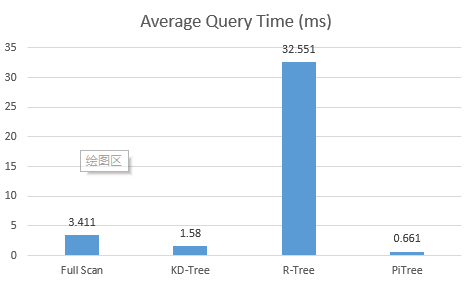
\includegraphics[width=.8\linewidth]{../figures/overall-performance/random-qtime} 
    \vspace{4ex}
  \end{minipage}%%
  \begin{minipage}[b]{0.33\linewidth}
    \centering
    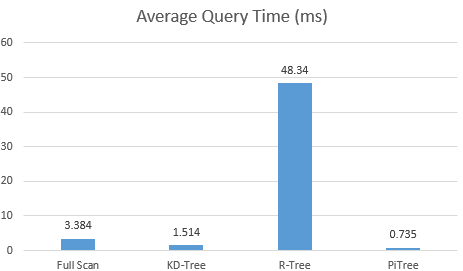
\includegraphics[width=.8\linewidth]{../figures/overall-performance/normal-qtime} 
    \vspace{4ex}
  \end{minipage}%%
  \begin{minipage}[b]{0.33\linewidth}
    \centering
    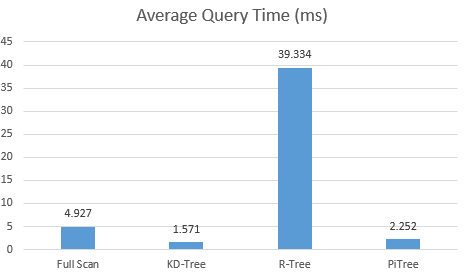
\includegraphics[width=.8\linewidth]{../figures/overall-performance/zipf-qtime} 
    \vspace{4ex}
  \end{minipage}
  \caption{Average query time for random, normal and zipf distribution (from left to right). 
  All datasets has a dimension of 2 and a selectivity of 0.1}
\end{figure*}

\begin{figure*}[t] 
  \label{overall-performance-btime} 
  \begin{minipage}[b]{0.33\linewidth}
    \centering
    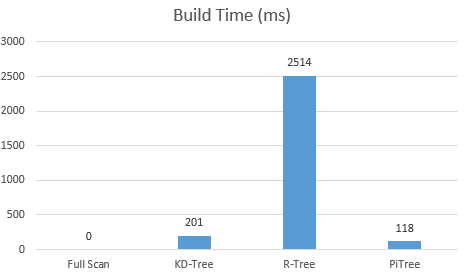
\includegraphics[width=.8\linewidth]{../figures/overall-performance/random-btime} 
    \vspace{4ex}
  \end{minipage}%%
  \begin{minipage}[b]{0.33\linewidth}
    \centering
    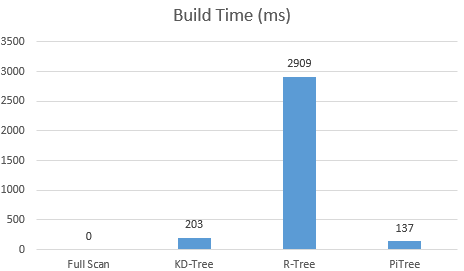
\includegraphics[width=.8\linewidth]{../figures/overall-performance/normal-btime} 
    \vspace{4ex}
  \end{minipage}%%
  \begin{minipage}[b]{0.33\linewidth}
    \centering
    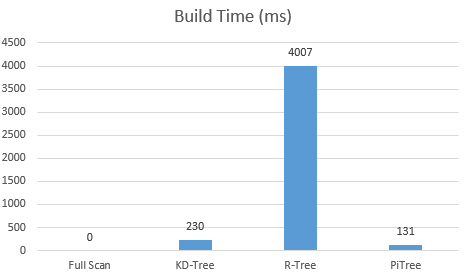
\includegraphics[width=.8\linewidth]{../figures/overall-performance/zipf-btime} 
    \vspace{4ex}
  \end{minipage}
  \caption{Average build time for random, normal and zipf distribution (from left to right). 
  All datasets has a dimension of 2 and a selectivity of 0.1}
\end{figure*}

\subsection{Datasets}

\begin{table}[h]
  \centering
  \begin{tabular}{|c|c|c|c|c|}
    \hline
          & records & queries & dimension & selectivity \\
    \hline
    random & 1M & 1K & 2-20 & 0.0001 - 0.9 \\
    \hline
    normal & 1M & 1K & 2-20 & 0.0001 - 0.9 \\
    \hline
    zipf & 1M & 1K & 2 & 0.0001 - 0.1 \\
    \hline 
  \end{tabular}
  \caption{Dataset and query characteristics}
  \label{table:dataset}
\end{table}

Due to time constraints, we evaluate indexing structures only on synthetic datasets.
Table 2 summarizes the characteristics of datasets. Details are described as follow.
\begin{itemize}
  \item \textbf{Distributions}. We benchmark on three distributions, specifically the random uniform
  distribution, normal distribution and the zipfian distribution. The first two distributions
  widely exist in real world data patterns whereas zipfian distribution is commonly used in
  linguistics, insurance and the modeling of rare events.
  \item \textbf{Records}. Data records are randomly sampled from the corresponding distribution.
  We limit the number of records to 1M for fast loading and testing.
  \item \textbf{Queries}. For simplicity, each query selects on all dimensions. The start
  point is randomly from the distribution. An end point is selected in a way that the
  percentage of records falls into the interval equals to corresponding selectivity.
  \item \textbf{Dimension}. For each distribution, we generate records on dimension 2, 5, 10, 15,
  and 20 to test the scalability across dimensions of our indexing structures.
  \item \textbf{Selectivity}. Generating queries on high dimension with a fixed selectivity S is
  a hard problem. However, since each column is independent, the problem can be reduced to generate
  queries on each dimension with a selectivity of $S^{\frac{1}{D}}$. We generate queries with
  selectivity 0.0001, 0.001, 0.01, 0.1, 0.5 and 0.9 to test the scalability across selectivity.
\end{itemize}

\subsection{Overall Performance}

\begin{table}[h]
  \centering
  \begin{tabular}{|c|c|c|c|c|}
    \hline
          & full scan & KD-Tree & R-Tree & Pi-Tree \\
    \hline
    random & 0 & 78125 & 7843 & 78 \\
    \hline
    normal & 0 & 78125 & 7843 & 91 \\
    \hline
    zipf & 0 & 78125 & 7843 & 0.1 \\
    \hline 
  \end{tabular}
  \caption{Memory Usage KB}
  \label{table:mem}
\end{table}

%% TODO update plot title
\begin{figure*}[ht] 
  \label{overall-performance-qtime} 
  \begin{minipage}[b]{0.33\linewidth}
    \centering
    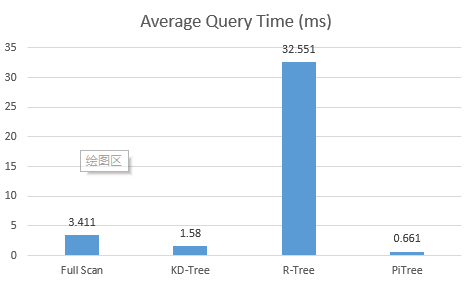
\includegraphics[width=.8\linewidth]{../figures/overall-performance/random-qtime} 
    \vspace{4ex}
  \end{minipage}%%
  \begin{minipage}[b]{0.33\linewidth}
    \centering
    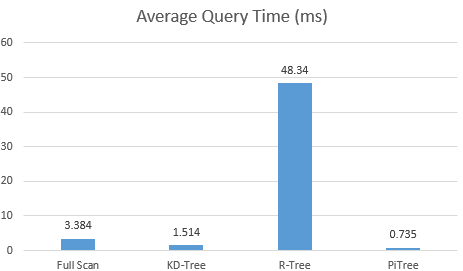
\includegraphics[width=.8\linewidth]{../figures/overall-performance/normal-qtime} 
    \vspace{4ex}
  \end{minipage}%%
  \begin{minipage}[b]{0.33\linewidth}
    \centering
    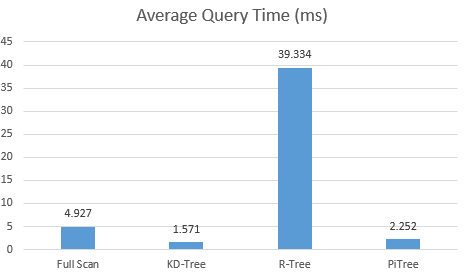
\includegraphics[width=.8\linewidth]{../figures/overall-performance/zipf-qtime} 
    \vspace{4ex}
  \end{minipage}
  \caption{Average query time for random, normal and zipf distribution (from left to right). 
  All datasets has a dimension of 2 and a selectivity of 0.1}
\end{figure*}

\begin{figure*}[ht] 
  \label{overall-performance-btime} 
  \begin{minipage}[b]{0.33\linewidth}
    \centering
    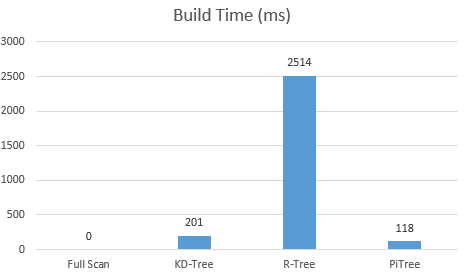
\includegraphics[width=.8\linewidth]{../figures/overall-performance/random-btime} 
    \vspace{4ex}
  \end{minipage}%%
  \begin{minipage}[b]{0.33\linewidth}
    \centering
    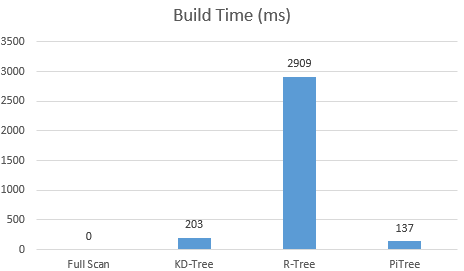
\includegraphics[width=.8\linewidth]{../figures/overall-performance/normal-btime} 
    \vspace{4ex}
  \end{minipage}%%
  \begin{minipage}[b]{0.33\linewidth}
    \centering
    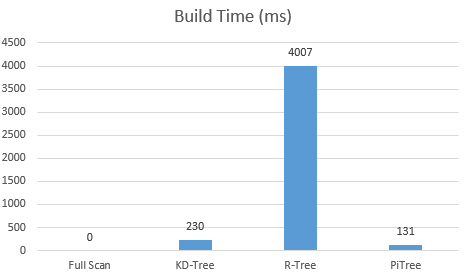
\includegraphics[width=.8\linewidth]{../figures/overall-performance/zipf-btime} 
    \vspace{4ex}
  \end{minipage}
  \caption{Average build time for random, normal and zipf distribution (from left to right). 
  All datasets has a dimension of 2 and a selectivity of 0.1}
\end{figure*}

We first benchmark the building time, memory usage and query speed of Pi-Tree against
other indexing structures under 3 distributions. Figure 4 shows the average query time of
Pi-Tree is 2-3 times faster than the next closest indexing structure. Pi-Tree is surpassed by
KD-Tree under zipfian distribution where data is highly skewed and cannot be learned effectively
by linear regression. A print of Pi-Tree shows that it tries to learn the whole distribution
with a single node which results in large prediciton errors.

In terms of memory usage (see Table 3), Pi-Tree is able to reduce the memory usage by 2-3 orders of magnitude
since it significantly reduces the depth of the tree by utilitizing linear regression with fanout and
page size. The size of Pi-Tree various across different distributions as it will learn a reasonable number
of nodes for a particular distribution. In Table 3, the size of Pi-Tree is only 0.1KB for zipf
distribution as it only creates one node for the whole distribution. Pi-Tree is also able to load data and build the tree 2 times faster than KD-Tree and over 20 times
faster than R-Tree as shown in Figure 5. Such building time is independent from distributions.

Figure 6 shows the prediction error distribution that helps to understand the performance
difference of Pi-Tree under different distributions. It's not suprising to see that Pi-Tree
models random uniform distribution best with an error bounded by 25 entries. The error under
normal distribution is also reasonable and can be corrected within several steps of quadratic
search. While the error for zipfian distribution goes beyond 300 entries and results in the
search speed to be 3 times slower.

\begin{figure}[h]
  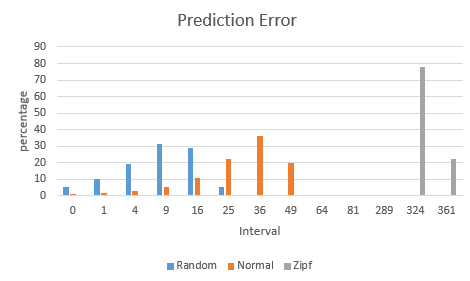
\includegraphics[scale=0.6]{../figures/addition/prediction-error}
  \caption{Prediction error}
  \label{prediction-error}
\end{figure}

\subsection{Scalability}

To show the scalability of PiTree, we benchmark our indexing structures on different
query selectivities and dimensions. The results show that our PiTree is robust to the
scale of query selectivity and dimensions.

\subsubsection{Query Selectivity}

\begin{figure*}[ht] 
  \label{scalability-selectivity} 
  \begin{minipage}[b]{0.45\linewidth}
    \centering
    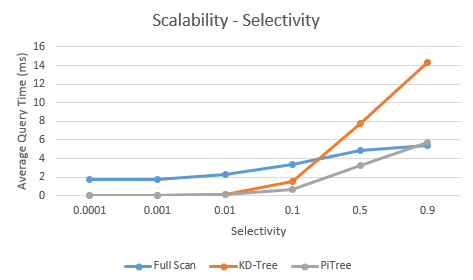
\includegraphics[width=.8\linewidth]{../figures/scalability/selectivity-random} 
    \vspace{4ex}
  \end{minipage}%%
  \begin{minipage}[b]{0.45\linewidth}
    \centering
    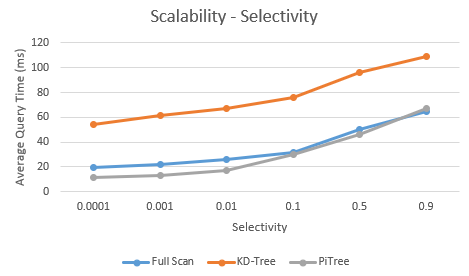
\includegraphics[width=.8\linewidth]{../figures/scalability/selectivity-normal} 
    \vspace{4ex}
  \end{minipage}%%
  \caption{Average query time under different selectivities. Left figure is tested
  on 2D random distribution while right figure is tested on 20D normal distribution.
  Results of R-Tree are excluded since they are 20 times slower than others.}
\end{figure*}

Figure 7 shows the benchmark results under different selectivities where we fixed the
distribution as 2D random and 20D normal respectively. Results of R-Tree are excluded
as they are 20 times slower.

PiTree remains to be the fastest until selectivity goes more than 50\%. Under high selectivity,
full scan outperformes others as indexing structures cannot prune effectively and scanning
time becomes the dominant part in lookup. The performance of both PiTree and KD-Tree degrades
as selectivity increasing, but KD-Tree is more vulnerable to selectivity changes.

\subsubsection{Dimension}

\begin{figure*}[ht] 
  \label{scalability-dimension} 
  \begin{minipage}[b]{0.45\linewidth}
    \centering
    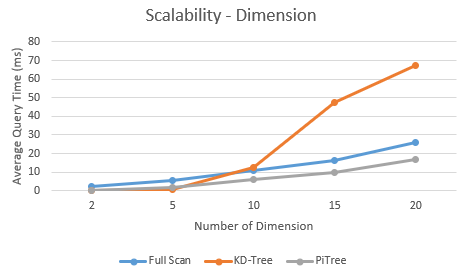
\includegraphics[width=.8\linewidth]{../figures/scalability/dimension-random} 
    \vspace{4ex}
  \end{minipage}%%
  \begin{minipage}[b]{0.45\linewidth}
    \centering
    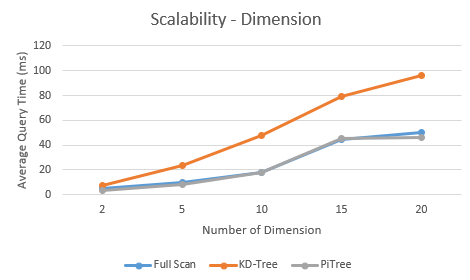
\includegraphics[width=.8\linewidth]{../figures/scalability/dimension-normal} 
    \vspace{4ex}
  \end{minipage}%%
  \caption{Average query time under different dimensions. Left figure is tested
  on random distribution with 0.01 selectivity while right figure is tested on normal distribution
  with 0.5 selectivity.
  Results of R-Tree are excluded since they are 20 times slower than others.}
\end{figure*}

We first benchmark the building time, memory usage and query speed of Pi-Tree against
other indexing structures under 3 distributions. Figure 4 shows the average query time of
Pi-Tree is 2-3 times faster than the next closest indexing structure. Pi-Tree is beated by
KD-Tree under zipfian distribution where data is highly skewed and cannot be learned effectively
by linear regression. A print of Pi-Tree shows that it tries to learn the whole distribution
with a single node which results in large prediciton errors.

In terms of memory usage (see Table 3), Pi-Tree is able to reduce the memory usage by 2-3 order of magnitude
since it significantly reduce the depth of the tree by utilitizing linear regression with fanout and
page size. The size of Pi-Tree various across different distributions as it will learn a reasonable number
of node for a particular distribution. In Table 3, the size of Pi-Tree is only 0.1KB for zipf
distribution as it only create one node for the whole distribution. Pi-Tree is also able to load data and build the tree 2 times faster than KD-Tree and over 20 times
faster than R-Tree as shown in Figure 5. Such building time is independent from distributions.

Figure 6 shows the prediciton error distribution that helps to understand the performance
difference of Pi-Tree under different distributions. It's not suprising to see that Pi-Tree
models random uniform distribution best with an error bounded by 25 entries. The error under
normal distribution is also reasonable and can be corrected within several steps of quadratic
search. While the error for zipfian distribution goes beyond 300 entries and results in the
search speed to be 3 times slower.

\begin{figure*}[ht] 
  \label{parameter-fix-pageSize} 
  \begin{minipage}[b]{0.33\linewidth}
    \centering
    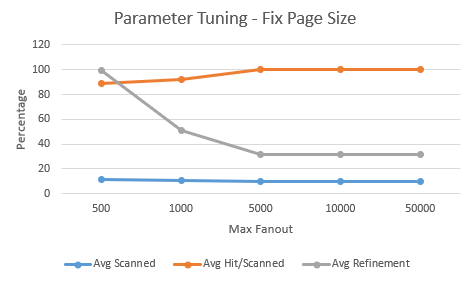
\includegraphics[width=.8\linewidth]{../figures/parameter/fix-pagesize-hit} 
    \vspace{4ex}
  \end{minipage}%%
  \begin{minipage}[b]{0.33\linewidth}
    \centering
    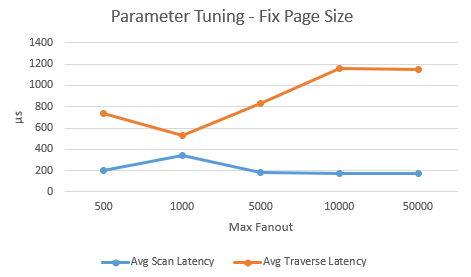
\includegraphics[width=.8\linewidth]{../figures/parameter/fix-pagesize-latency} 
    \vspace{4ex}
  \end{minipage}%%
  \begin{minipage}[b]{0.33\linewidth}
    \centering
    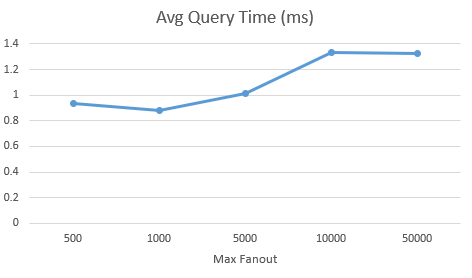
\includegraphics[width=.8\linewidth]{../figures/parameter/fix-pagesize-qtime} 
    \vspace{4ex}
  \end{minipage}
  \caption{Statistics collected by changing max fanout. Test on 2D random distribution
  with a fixed page size of 1000}
\end{figure*}

Figure 9 shows the statistics collected by changing the max fanout. Both average
hit ratio and refinement ratio become stable after max fanout reaches 5000. While
the average tree traverse latency, which represents the effectiveness of pruning,
first reaches a sub-optimal point and start to increase together with the max fanout.
This results in a higher average query time as shown in the right most picture of Figure 9.

\subsubsection{Page Size}

\begin{figure*}[ht] 
  \label{parameter-fix-fanout} 
  \begin{minipage}[b]{0.33\linewidth}
    \centering
    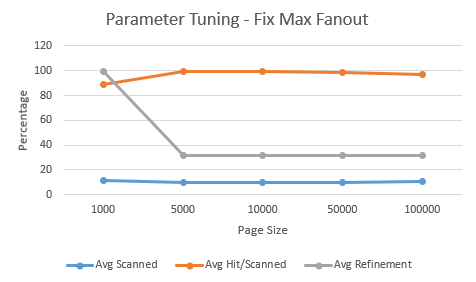
\includegraphics[width=.8\linewidth]{../figures/parameter/fix-fanout-hit} 
    \vspace{4ex}
  \end{minipage}%%
  \begin{minipage}[b]{0.33\linewidth}
    \centering
    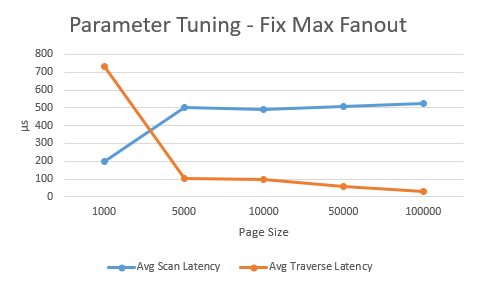
\includegraphics[width=.8\linewidth]{../figures/parameter/fix-fanout-latency} 
    \vspace{4ex}
  \end{minipage}%%
  \begin{minipage}[b]{0.33\linewidth}
    \centering
    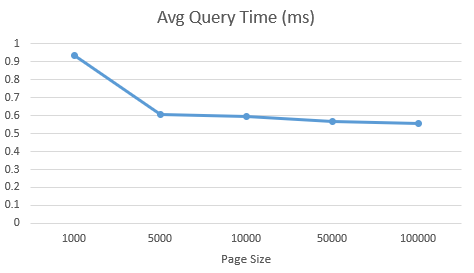
\includegraphics[width=.8\linewidth]{../figures/parameter/fix-fanout-qtime} 
    \vspace{4ex}
  \end{minipage}
  \caption{Statistics collected by changing page size. Test on 2D random distribution
  with a fixed max fanout of 500}
\end{figure*}

\subsection{Scalability}

To show the scalability of PiTree, we benchmark our indexing structures on different
query selectivities and dimensions. The results show that our PiTree is robust to the
scale of query selectivity and dimensions.

\subsubsection{Query Selectivity}

Figure 7 shows the benchmark results under different selectivities where we fixed the
distribution as 2D random and 20D normal respectively. Results of R-Tree are excluded
as they are 20 times slower.

PiTree remains to be the fastest until selectivity goes more than 50\%. Under high selectivity,
full scan outperformes others as indexing structures cannot prune effectively and scanning
time becomes the dominant part in lookup. The performance of both PiTree and KD-Tree degrades
as selectivity increasing, but KD-Tree is more vulnerable to selectivity changes.

\subsubsection{Dimension}

Figure 8 shows the benchmark results under different dimensions where we fixed the
distribution as random distribution with 0.01 selectivity and normal distribution with
0.5 selectivity. Results of R-Tree are omitted for similar reason as above.

As number of dimensions increases, the performance of KD-Tree degrades dramatically as
the depth of the tree grows quickly. The query time of both PiTree and full scan increases
linearly along with dimensions while PiTree remains to be the fastest indexing structure.

\subsection{Parameter Tuning}

This section studies the influence parameters used in PiTree (i.e. max fanout and page size)
which is intented to guide our future work on cost model.

\subsubsection{Max Fanout}

Figure 9 shows the statistics collected by changing the max fanout. Both average
hit ratio and refinement ratio become stable after max fanout reaches 5000. While
the average tree traverse latency, which represents the effectiveness of pruning,
first reaches a sub-optimal point and start to increase together with the max fanout.
This results in a higher average query time as shown in the right most picture of Figure 9.

\subsubsection{Page Size}

Figure 10 shows the statistics collected by changing the page size which shows
a similar trend as changing the max fanout in Figure 9 since a better partition
can be achieved by either increasing the page size or tuning the max fanout. As
the page size increases, average scan latency also increases because there more
records to scan within each page while average tree traverse latency decreases
and eventually leads to a faster query speed.

\subsubsection{Combined View}

Figure 11 shows a combined view of the influence of page size and max fanout towards
average query time. Although larger max fanout and page size yields better query speed
in general, the optimal parameter is 50K page size and 1K max fanout which falls in
the middle. Therefore, a better idea is to solve the parameters as an optimization
problem as described in section 7.

\begin{figure}
  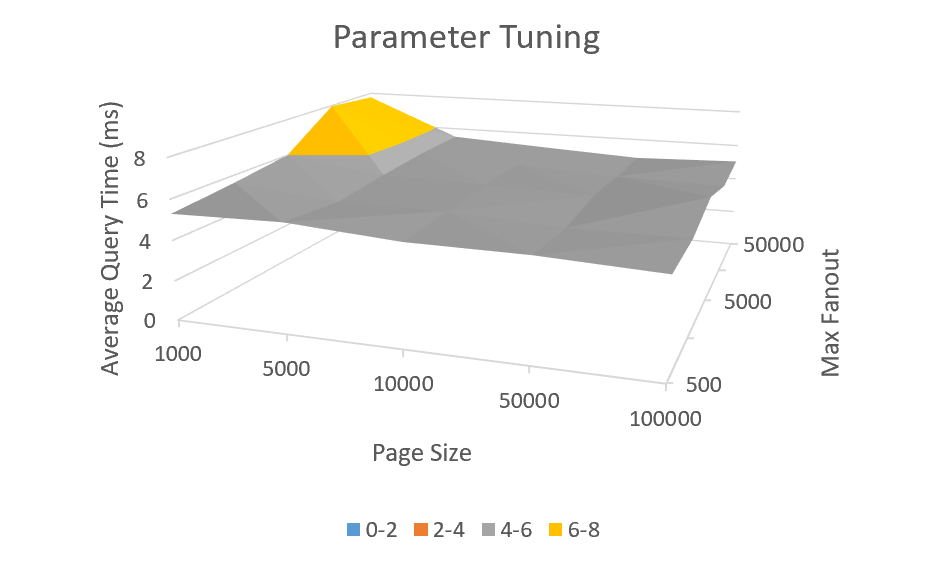
\includegraphics[scale=0.6]{../figures/parameter/avg-qtime-3D2}
  \caption{Average query time with various max fanout and page size}
  \label{combined-view}
\end{figure}

\section{Future Work}

Due to time constaints there are a few things
that we wanted to explore but did not have time.
Most importantly, we wanted to explore using different
projection selection policies, and in particular using
non-axis aligned policies to account for non-independent dimensions.
Most work in databases assumes independence between columns,
for example for cost estimation in the query optimizer \cite{SelectivityEstimation}.
Incorporating off-axis projection could theoretically better model 
correlated dimensions.

One policy that could produce off-axis projections is using
Principal Component Analysis (PCA). The idea would be to 
pick the first princiapl component which is the projection that captures
the maximum possible variance in the data.

Another idea is to incorporate cost model to determine how the tree is built.
Currently, Pi-Tree uses two paramters and a simple heuristic to determine
if a node should be a leaf and the fanout of internal nodes.
Further exploration could be done on how to better determine the ideal
fanout of each node.

\section{Conclusion}

This paper has presented the design of a simple,
novel, performant, multidimensional learned index strucutre.

%%
%% The acknowledgments section is defined using the "acks" environment
%% (and NOT an unnumbered section). This ensures the proper
%% identification of the section in the article metadata, and the
%% consistent spelling of the heading.
\begin{acks}
Adam wants to thank his girlfriend Akshaya for always being there and
helping out.
\end{acks}

%%
%% The next two lines define the bibliography style to be used, and
%% the bibliography file.
\bibliographystyle{ACM-Reference-Format}
\bibliography{refs.bib}


\end{document}
\endinput
%%